\section{Background}

Reinforcement learning (RL) algorithms have been used to align Large Language Models (LLMs) with human preferences (RLHF) and to optimize verifiable reward signals (RLVR; e.g., \cite{RLVR,GRPO}). 

\subsection{Policy Gradient and the REINFORCE Algorithm}
The foundational method for this optimization is the policy gradient theorem~\cite{REINFORCE,rlbook}. For LLMs, a trajectory consists of generating a single response $y$ from a prompt $x$. The objective function is the expected reward:
\begin{equation}
    J(\theta) = \mathbb{E}_{x \sim \mathcal{D}, y \sim \pi_\theta(\cdot|x)}[R(x,y)],
\end{equation}
where $\mathcal{D}$ is the prompt distribution and $R(x,y)$ is the reward for generating response $y$ for prompt $x$. The gradient of this objective is given by:
\begin{equation}
    \nabla_\theta J(\theta) = \mathbb{E}_{x \sim \mathcal{D}, y \sim \pi_\theta(\cdot|x)}[R(x,y) \nabla_\theta \log \pi_\theta(y|x)].
\end{equation}
This formulation gives rise to the REINFORCE algorithm~\cite{REINFORCE,rlbook}, which updates the policy by taking a step in the direction of this estimated gradient. A significant drawback of REINFORCE is the high variance of its gradient estimator. The raw reward $R(x,y)$ can fluctuate widely, leading to noisy updates and unstable training.

To mitigate high variance, a baseline $b(x)$ that is conditionally independent of the action $y$ can be subtracted from the reward. This results in an unbiased gradient estimator with provably lower variance~\cite{greensmith2004variance}:
\begin{equation}
    \nabla_\theta J(\theta) = \mathbb{E}_{x \sim \mathcal{D}, y \sim \pi_\theta(\cdot|x)}[(R(x,y) - b(x)) \nabla_\theta \log \pi_\theta(y|x)].
\end{equation}
The term $A(x,y) = R(x,y) - b(x)$ is known as the advantage. The optimal baseline that minimizes variance is the true value function $V_\pi(x) = \mathbb{E}_{y \sim \pi_\theta(\cdot|x)}[R(x,y)]$, which is the expected reward for a given prompt $x$. In practice, $V_\pi(x)$ is unknown and must be estimated. The quality of this estimation is crucial for the stability and efficiency of the RL algorithm.

\subsection{Variance Reduction Baselines for Large Language Models}
Several strategies have been developed to estimate the baseline $b(x)$ in the context of LLM training. PPO~\cite{PPO} trains a parameterized critic network $v_\phi$. However, learning $v_\phi$ is notoriously unstable and resource-intensive, as $\phi$ typically matches the size of the LLM policy parameters $\theta$.

A common approach is to construct an empirical, on-the-fly baseline from multiple samples. Group Relative Policy Optimization (GRPO)~\cite{GRPO,R1} generates a group of $G$ responses $\{y_1, \dots, y_G\}$ for a single prompt $x$, then uses the mean rewards of the group as the baseline $b_\text{GRPO}$. Another popular baseline is the Leave-One-Out (RLOO). For a given sample $y_i$, the baseline is the average reward of the other $G-1$ samples in the group, denoted as $b_\text{RLOO}$:
\begin{equation}
        b_{\text{GRPO}}(x) = \frac{1}{G} \sum_{j} R(x, y_j),  \qquad
    b_{\text{RLOO}}(x,y_i) = \frac{1}{G-1} \sum_{j \neq i} R(x, y_j).
\end{equation}

The \emph{raw} advantage for sample $y_i$ is then $A(x, y_i) = R(x,y_i) - b_{\text{GRPO}}(x)$, then it is normalized with the standard deviation $\sigma_G$. While simple to implement, this approach suffers from two key limitations. First, it is sample-inefficient, requiring $G>1$ generations per prompt for each gradient step. Second, the baseline is estimated from a very small group ($G$), making it a high-variance estimate of the true value function, which in turn leads to noisy advantage estimates.


\section{Method}

We introduce Single-stream Policy Optimization (SPO), a method designed for policy optimization in settings with verifiable feedback (RLVR)~\cite{RLVR}. We assume the feedback is binary\footnote{Generalizing to non-binary rewards is straightforward, as discussed at the end of Section~\ref{sec:tracker}.}, i.e., $+1$ for success and $0$ for failure. SPO addresses the challenge of estimating a non-stationary success probability for a policy that evolves over training iterations. It integrates a Bayesian value tracker with an adaptive memory mechanism into a policy gradient framework. The core components are: (1) a KL-adaptive tracker that provides a low-variance, single-sample estimate of the success probability; (2) a global advantage normalization scheme that ensures high sample efficiency and stable learning dynamics; and (3) prioritized sampling across training prompts to focus on prompts with high learning potential. The following subsections detail each component.

\subsection{A KL-Adaptive Value Tracker}\label{sec:tracker}
The definition of a value function is the \emph{expected} reward of the prompt $x$ under policy $\pi$, i.e., $V_\pi(x) = \mathbb{E}_{y \sim \pi(\cdot|x)}[R(x,y)]$. We use \(\hat{v}(x)\) to denote the tracker’s running estimate of $V_\pi(x)$; that is, \(\hat{v}(x) \approx V_\pi(x)\). 
To estimate the non-stationary success probability of a prompt $x$, we use a Bayesian \emph{tabular} tracker instead of a separate value network\footnote{The development of core RL algorithms was on tabular representation~\cite{rlbook}.}. For the binary success/failure rewards common in RLVR, this is elegantly modeled using a Beta distribution, which is the conjugate prior for the Bernoulli process governing the outcomes. We therefore model the success probability $\hat{v}(x)$ using a Beta distribution: $\hat{v}(x) \sim \text{Beta}(\alpha(x), \beta(x))$, where the value estimate is the posterior mean $\hat{v}(x) = \alpha(x) / (\alpha(x) + \beta(x))$.

The tracker adapts to policy changes by dynamically adjusting its memory of past rewards. When the policy changes significantly, older observations become less relevant and should be downweighted. After each new observation $r(x, y) \in \{0, 1\}$, we discount the prior Beta parameters $(\alpha_{-1}, \beta_{-1})$ by a factor $\rho(x)$ before incorporating the new evidence $r(x,y)$:
\begin{equation}
    \alpha(x) = \rho(x) \alpha_{-1}(x) + r(x, y),  \quad 
    \beta(x)  = \rho(x) \beta_{-1}(x) + (1 - r(x, y)), \quad \hat{v}(x) = \frac{\alpha(x)}{\alpha(x) + \beta(x)}.
\end{equation}
The discount factor $\rho(x) = 2^{-D(x) / D_\text{half}}$ is determined by the KL divergence $D(x)$ between the current policy and the last policy that \emph{acted} on prompt $x$, causing the tracker to forget faster as the policy changes more significantly. The hyperparameter $D_\text{half}$ controls this forgetting rate $\rho \in [\rho_\text{min}, \rho_\text{max}]$.

\textbf{Initialization.} To initialize, we collect $n_0$ samples to compute an initial value estimate $\hat{v}_{0}(x)$. To avoid transient instability, we set the initial effective sample size to its expected equilibrium, $N_0 = 1 / (1 - \rho_{\min})$, where $\rho_{\min}$ is the minimum allowed forgetting factor. The initial parameters are then:
\begin{equation}
\alpha_0(x) = N_0 \cdot \hat{v}_{0}(x),  \qquad \beta_0(x) = N_0 \cdot (1 -\hat{v}_{0}(x)).
\end{equation}

This Bayesian update is equivalent to an adaptive Exponential Moving Average (EMA) on the value estimate:
\begin{equation}\hat{v}(x) = \hat{v}_{-1}(x) + \eta(x) (r(x, y) - \hat{v}_{-1}(x)),
\end{equation} 
where the learning rate $\eta(x) = (\rho(x) N_{\text{eff},-1}(x) + 1)^{-1}$ naturally adapts to both policy shifts (via $\rho(x)$) and statistical confidence (via $N_\text{eff} = \alpha(x) + \beta(x) + 1$). This formulation highlights how our tracker balances new evidence against accumulated knowledge. For \emph{general rewards} beyond binary ones, we can just use the same EMA formulation to directly track $\hat{v}$, rather than relying on $\alpha$ and $\beta$ in the binary cases.

\subsection{Advantage Estimation and Policy Optimization}

SPO uses the tracker's estimate $\hat{v}$ as a baseline for advantage calculation in a policy gradient algorithm. At iteration $i$, for a single reward $r(x, y)$ obtained with policy $\pi_{\theta_i}$, the advantage is computed using the \emph{pre-update} baseline (denoted with subscript $_{-1}$):
\begin{equation}
    A(x, y) = r(x, y) - \hat{v}_{-1}(x).
\end{equation}
Using the baseline from the previous step ensures that it is independent of the action taken at step $i$, preserving the unbiasedness of the policy gradient estimate. While the reward $r(x, y)$ is typically a direct outcome signal, SPO's framework is also compatible with more sophisticated reward functions. For instance, recent work like InfAlign~\cite{balashankar2024infalign} demonstrates how to calibrate and transform the reward signal to be ``inference-aware,'' directly optimizing for procedures like Best-of-$N$ sampling. Such transformed rewards can be seamlessly integrated into SPO by replacing the standard $r(x, y)$ in the advantage calculation. Since $v_{-1}(x)$ is independent of $y \sim \pi_{\theta_i}(\cdot| x)$, $\mathbb{E}\!\left[(r - v_{i-1}(x))\,\nabla_\theta \log \pi\right] = \nabla J(\theta)$~\cite{REINFORCE}. Instead of normalizing advantages on a per-prompt basis in a group~\cite{GRPO,R1}, SPO normalizes them across an entire batch of prompts $\mathcal{B}$~\cite{RFplusplus,PPO,andrychowicz2020matters,gem}.  The normalized advantage $\tilde{A}(x, y)$ is computed as:
\begin{equation}
    \tilde{A}(x, y) = \frac{A(x, y) - \mu_{\mathcal{B}}}{\sigma_{\mathcal{B}}},
\end{equation}
where $\mu_{\mathcal{B}}$ and $\sigma_{\mathcal{B}}$ are the mean and standard deviation of advantages in the batch $\{A(x, y)\}_{x \in \mathcal{B}}$. We then apply the advantage $\tilde{A}(x, y)$ to each \emph{token} in the response sequence $y$ and update the policy parameters using a standard PPO-Clip policy loss~\cite{PPO}{\footnote{The term ``PPO'' is frequently used with ambiguity. It may denote the entire algorithm suite (e.g., clipped policy and value losses), refer narrowly to just the clipped policy objective, or describe the broader training framework, including mechanisms like mini-batch updates.}:
\begin{align}
L^{\text{CLIP}}(\theta) &= \mathbb{E}_{s, t}\!\left[\min\!\Bigg(
\frac{\pi_\theta(a_t\mid s_t)}{\pi_{\theta_{\text{old}}}(a_t\mid s_t)}\,\tilde{A_t},\;
\operatorname{clip}\!\Big(\frac{\pi_\theta(a_t\mid s_t)}{\pi_{\theta_{\text{old}}}(a_t\mid s_t)},\,1-\varepsilon,\,1+\varepsilon\Big)\,\tilde A_t
\Bigg)\right]. 
\end{align}
Methods like Clip-Higher~\cite{DAPO}, Clip-Cov~\cite{cui2025entropy} and KL-Cov~\cite{cui2025entropy} to retain policy entropy are applicable here. Other policy optimization algorithms like CISPO~\cite{CISPO} (similar to \texttt{vtrace}~\cite{espeholt2018impala,wu2025llamarl}) and GSPO~\cite{GSPO} (use sequence-level likelihood instead of token-level) are compatible with our advantage estimator. Advanced methods to control policy behaviors like ASPO~\cite{aspo} can be utilized to modulate the advantage values. We note that if we use ``no baseline'' (i.e., $\hat{v} = 0$), it is an extremely simple and valid algorithm but may suffer from high policy gradient variance.

\subsection{Prioritized Prompt Sampling}

\begin{algorithm}[t]
\caption{Single-stream Policy Optimization}
\label{alg:SPO-train}
\begin{algorithmic}[1]
\For{iteration $i = 1, 2, \dots, T$}
    \State For each $x \in \mathcal{X}$, compute sampling weight $w_i(x)$ according to Eqn.~(\ref{eqn:sampling_coef}).
    \State Sample a batch of $B$ prompts $\mathcal{B}_i \subset \mathcal{X}$ according to weights $\{w_i(x)\}$.
    \State $\mathcal{D} \gets \emptyset$
    \For{each prompt $x \in \mathcal{B}_i$}
        \State Sample action $y \sim \pi_{\theta_{i-1}}(\cdot \mid x)$ and observe reward $r(x, y) \in \{0,1\}$.
        \State Compute raw advantage $A(x, y) \gets r(x, y) - \hat{v}_{-1}(x)$. \hfill %
        \State Store $(x, y, A(x, y))$ in $\mathcal{D}$.
        \State Update tracker $\hat{v}(x)$.
    \EndFor
    \State Normalize advantages: $\tilde{A}(x, y) \gets \big(A(x, y) - \mu_{\mathcal{B}_i}\big) / \sigma_{\mathcal{B}_i}$.
    \State Update $\theta_{i-1}$ to $\theta_i$ using mini-batches with a policy gradient algorithm (e.g., PPO-Clip).
\EndFor
\end{algorithmic}
\end{algorithm}
To further enhance data efficiency, SPO employs a curriculum learning strategy by prioritizing prompts with the highest learning potential~\cite{schaul2015prioritized,rlbook}. 
At each iteration, we sample a batch of prompts based on a score that emphasizes prompts with high uncertainty, while ensuring a minimum level of exploration. 
The sampling weight $w_i(x)$ for prompt $x$ is defined as:
\begin{equation} \label{eqn:sampling_coef}
    w_i(x) \propto \sqrt{\hat{v}_{-1}(x)\bigl(1 - \hat{v}_{-1}(x)\bigr)} + \epsilon.
\end{equation}
The first term corresponds to the estimated standard deviation of a Bernoulli outcome, which naturally allocates more weight to prompts that are neither almost always solved ($\hat{v} \approx 1$) nor almost always failed ($\hat{v} \approx 0$). 
The exploration bonus $\epsilon$, set to $0.05$ by default, prevents curriculum collapse by ensuring that every prompt retains a non-zero probability of being sampled, thereby maintaining broad coverage of the data distribution.
The complete SPO training procedure is outlined in Algorithm~\ref{alg:SPO-train}.

\begin{figure}[h!]
    \centering
    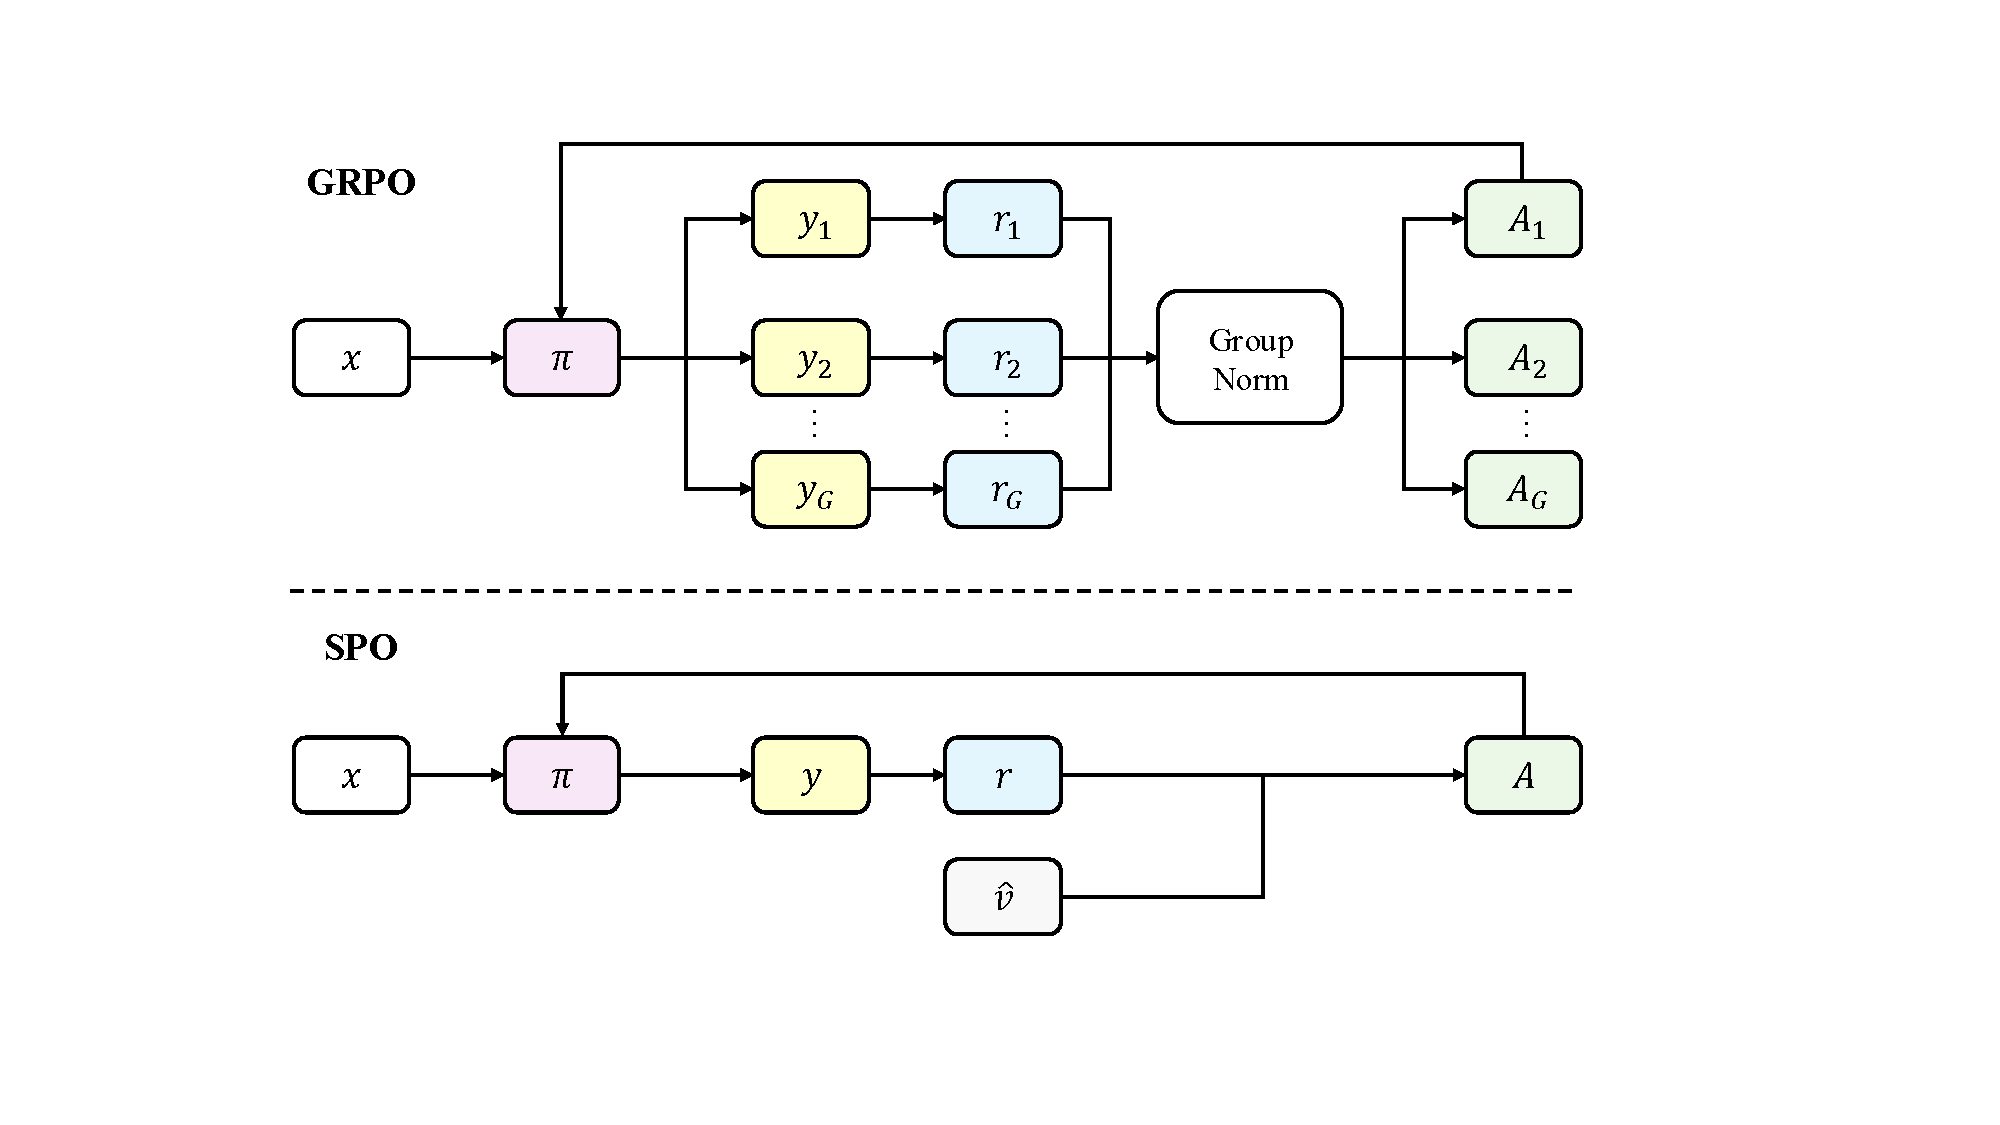
\includegraphics[width=0.6\linewidth]{figures/GRPO_vs_SPO.pdf}
    \caption{Illustrations of GRPO and the proposed SPO.}
    \label{fig:grpo_spo}
\end{figure}


\subsection{Advantages over GRPO}

\textbf{Group-Free for Scalable Infrastructure.}
SPO's design is inherently ``group-free'', a significant advantage in distributed training frameworks for LLMs. Each sample, consisting of a single stream of (prompt, response) pair, is a self-contained data point for the policy update. GRPO, however, requires the generation and evaluation of an entire group of $G$ samples for a single prompt before any training signal can be computed. We provide our illustrations in Figure~\ref{fig:grpo_spo}. In a distributed setting, this introduces a synchronization barrier: the processing of a given prompt is not complete until all $G$ responses have been generated. This is particularly problematic in the presence of long-tail generation times, where a single slow response generation can stall the processing for its \emph{entire group}. For constructing a training batch, SPO only needs to collect $B$ independent (prompt, response) pairs, which is far more flexible and efficient than waiting for $B$ entire groups to complete. This makes SPO's architecture significantly more infrastructure-friendly and scalable. The advantage is amplified in agentic training, especially in settings that require multi-turn interactions with tools~\cite{gao2025beyond, chen2025browsecomp} or long-horizon agent rollouts~\cite{zeng2025glm,xu2025agents}. The scale of these interactions can be substantial: state-of-the-art open-source models (\texttt{gpt-oss-120b}) may average 20~search turns per task~\cite{chen2025browsecomp}, with other agentic sessions reaching over 40~tool calls and generating up to 150,000 tokens of context~\cite{gao2025beyond}.

\textbf{Adaptive Curriculum.}
To further enhance training efficiency, SPO integrates a prioritized sampling scheme. This mechanism naturally creates an adaptive curriculum by focusing computational resources on prompts with the highest learning potential. This ensures that the model's training is concentrated on the most informative examples at any given point in time. GRPO, in its standard formulation, typically relies on uniform sampling of prompts. This may waste computation on prompts that are already mastered or are currently too difficult to yield useful learning signals. While dynamic sampling~\cite{DAPO} and repeat strategies~\cite{Polaris2025} have been proposed to mitigate this issue, they often discard samples \emph{after} generation, wasting computation. SPO’s prioritized sampling addresses the scheduling problem \emph{before} response generation, leading to a more natural and efficient training process. 

More discussions on the \emph{inefficiency} of dynamic sampling and the \emph{variance reduction} of policy gradient are outlined in Appendix~\ref{appendix:advanatages_over_GRPO}, where we provide detailed analysis.


